\documentclass{homework}
\usepackage{lipsum}
\usepackage{cancel}
\usepackage{amsthm}
\usepackage{cleveref}
\usepackage{upgreek}
\usepackage{mathrsfs}
\usepackage{tikz}
\usepackage{units}
\newtheorem{lemma}{Lemma}

\DeclareMathOperator{\cov}{cov}

\title{Kevin Joyce}
\course{Stat 542 - Applied Linear Models - Homework 4}
\author{Kevin Joyce}
\docdate{\today}
\begin{document} 
\newcommand{\figref}[1]{\figurename~\ref{#1}}
\renewcommand{\bar}{\overline}
\renewcommand{\hat}{\widehat}
\renewcommand{\SS}{\mathcal S}
\newcommand{\HH}{\mathscr H}
\newcommand{\mom}{\widetilde}
\newcommand{\mle}{\widehat \Uptheta}
\newcommand{\eps}{\varepsilon}
\newcommand{\todist}{\stackrel{D}\longrightarrow}
\newcommand{\toprob}{\stackrel{p}\longrightarrow}
\newcommand{\TTheta}{\overline{\underline \Theta} }
\newcommand{\del}{\partial}
\newcommand{\approxsim}{\overset{\cdotp}{\underset{\cdotp}{\sim}}}
\newcommand{\RSS}{\ensuremath{\mathrm{RSS}}}
\newcommand{\MSE}{\ensuremath{\mathrm{MSE}}}
\newcommand{\SE}{\ensuremath{\mathrm{SE}}}
\newcommand{\TSS}{\ensuremath{\mathrm{TSS}}}
\newcommand{\SSReg}{\ensuremath{\mathrm{SSReg}}}
\renewcommand{\a}[1]{{\color{red} \it #1}}


\begin{longproblem} Faraway 4.4.~(pg.~75) For the \texttt{swiss} data, fit a model with
\texttt{Fertility} as the response and the other variables as predictors. Perform regression diagnostics on the model to answer following questions.  Display any plots that are relevant.  Do not provide any plots about which you have nothing to say.
Also construct a half-normal plot of the
leverages and interpret the plot. 
\footnote{Codes for this homework are avaliable at \url{https://github.com/kjoyce/applied_linear_models/tree/master/homework04}}
\begin{enumerate}[(a)]
  \item Check the constant variance assumption for the errors.
  \item Check the normality assumption.
  \item Check for large leverage points.
  \item Check for outliers.
  \item Check for influential points.
  \item Check the structure of the relationship between the predictors and the response.
\end{enumerate}

\textbf{Solution: }

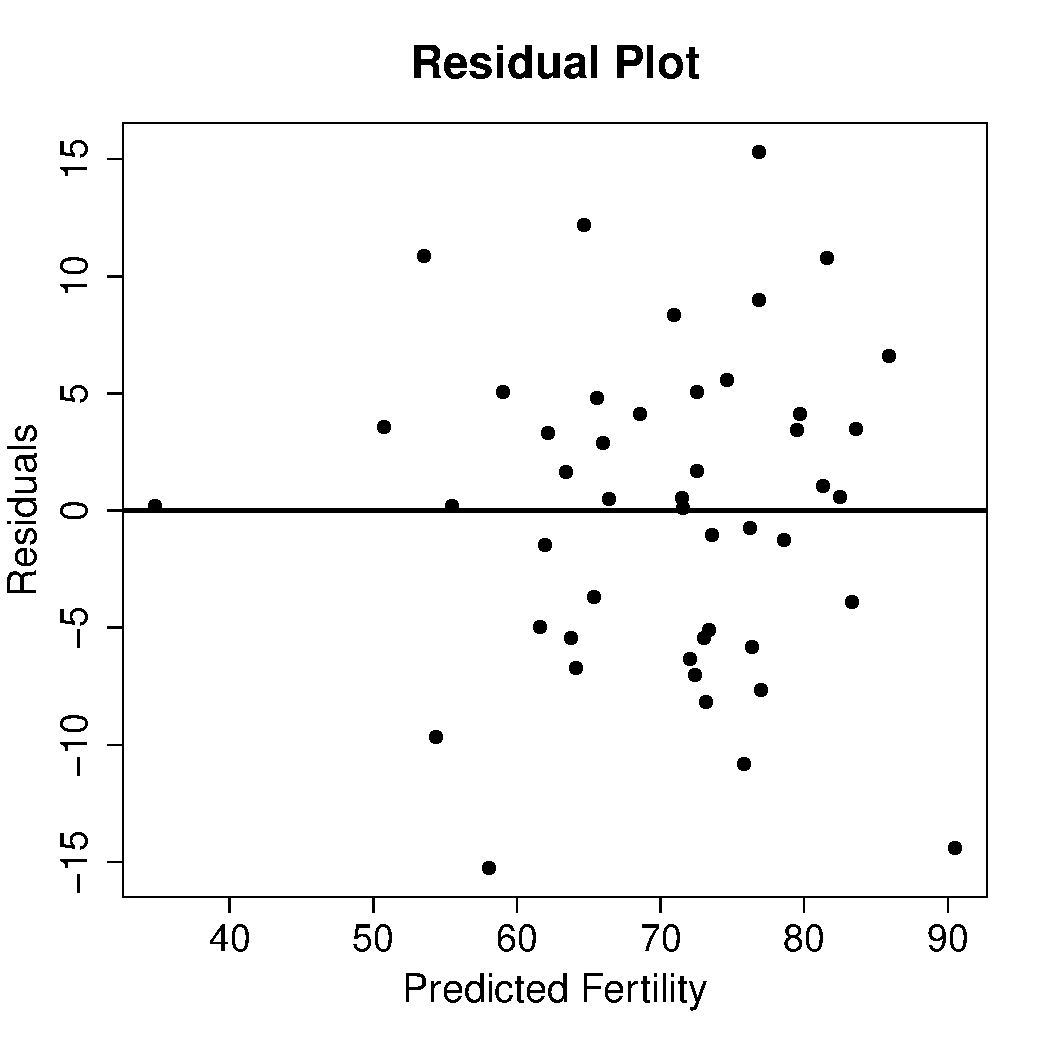
\includegraphics[width=.45\textwidth]{resid1.pdf}
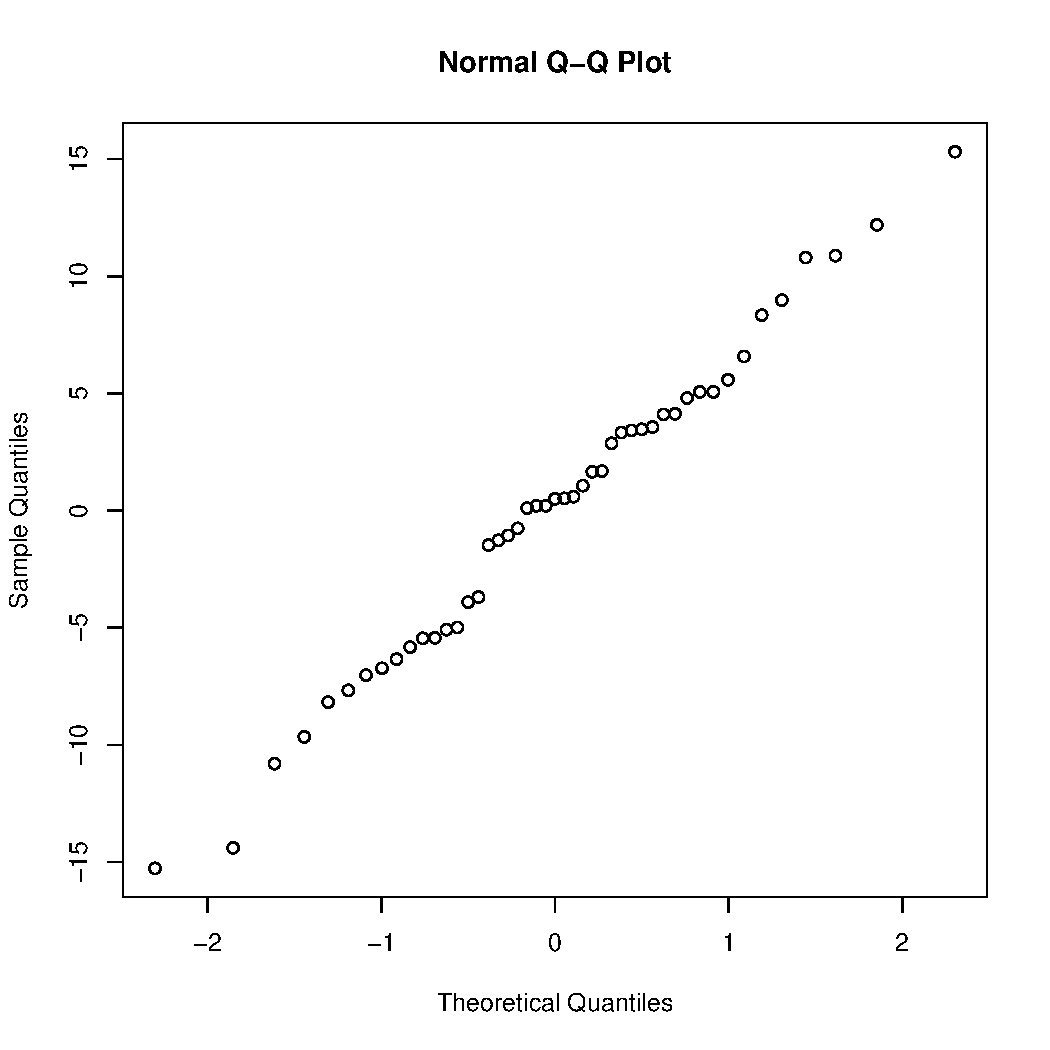
\includegraphics[width=.45\textwidth]{qqplot1.pdf}

\begin{minipage}{.4\textwidth}
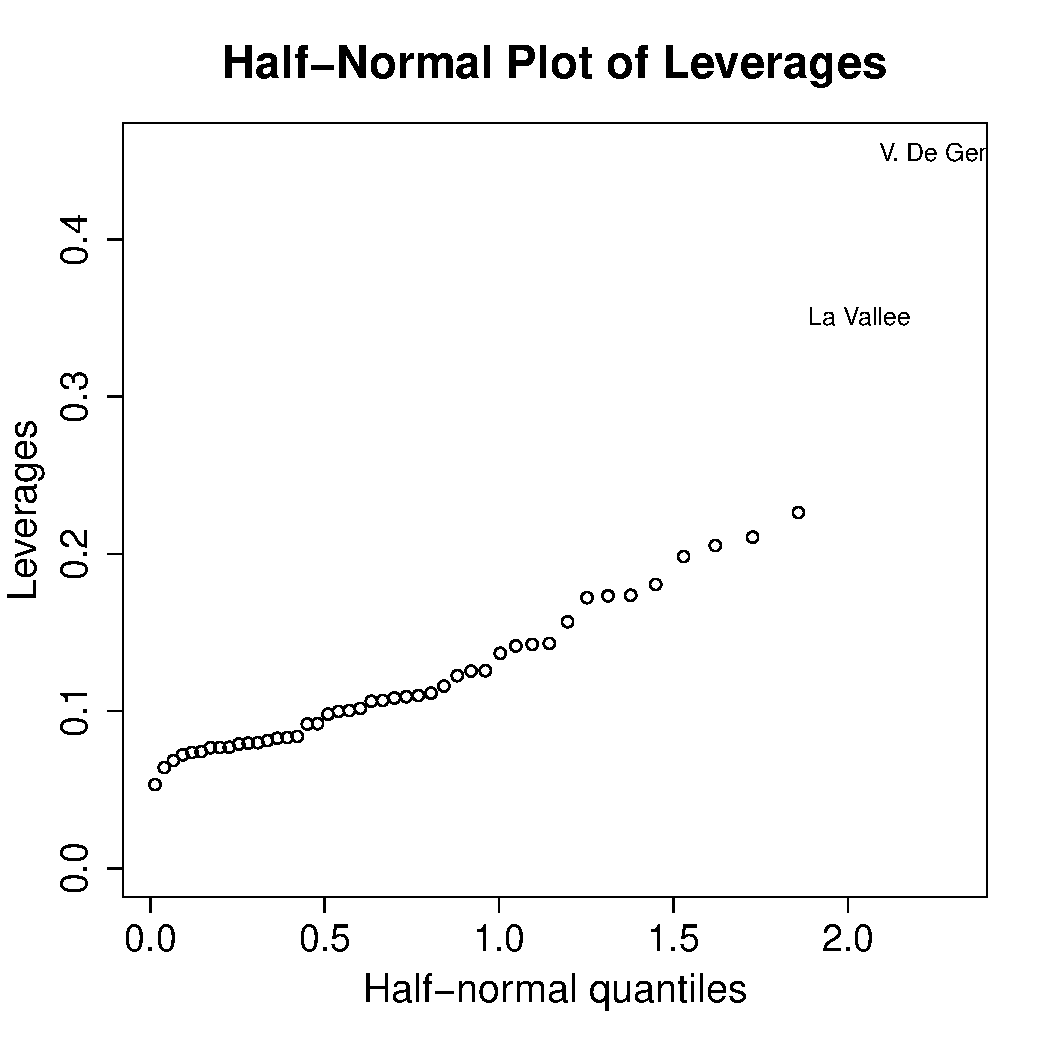
\includegraphics[width=\textwidth]{half-normal1.pdf}
\end{minipage}
\begin{minipage}{.6\textwidth}
\subproblem{ No discernible patterns are apparent in the residual plot (model residuals vs.~predicted fertility).}

\subproblem{ The qq-plot for normality reveals no evidence for non-normality.  This is confirmed by a Shapiro-Francia test: \texttt{W = 0.9901, p-value = 0.9087}.}

\subproblem{ Two potentially influential regions have leverage greater than $2p/n$: La Vellee with $h=0.351$ and V. De Geneve $h=0.456$.  Note that these values are indicated in the half-normal plot to the left.}
\end{minipage}

\subproblem{ Outliers were determined by testing the studentized deleted residual at the \%95 Bonferroni corrected level.  No observations had a residual that was greater than $t_{.05/2\cdot 47}(47-6-1)=3.529$. }

\subproblem{ Influential points were determined from those that had
high a leverage, or high Cook's D, DFFits, or DFBetas statistics.  Those
higher than the rubrics described in 5(d) are given below.}

{\small
\begin{tabular}{c | c c c c c c c c }
Obs & $h_i$ & Cooks D & DFFits & DF Ag. & DF Exam. & DF Educ. & DF Cath. & DF Inf. Mort. \\ \hline
Franches-Mnt  &0.174 &  0.036 &  0.463 &  \a{-0.349} & -0.218 &  -0.079 &  0.127 &  -0.104 \\
 Neuveville   & 0.072 &  0.041 &  0.507 &  0.033 &  \a{-0.303} & 0.291 &  \a{-0.390} & 0.136 \\
 Porrentruy   & 0.198 &  \a{0.208} &  \a{-1.177} &  \a{0.573} & 0.269 &  0.139 &  -0.256 &  \a{-0.659} \\
 Glane        & 0.141 &  0.073 &  0.674 &  0.226 &  0.281 &  -0.078 &  \a{0.308} & \a{0.422} \\
 La Vallee    & \a{0.351} &  0.034 &  0.451 &  -0.164 &  0.138 &  -0.150 &  0.127 &  \a{-0.373} \\
 Sierre       & 0.142 &  \a{0.148} &  \a{0.997} &  0.088 &  \a{-0.298} & 0.089 &  0.207 &  \a{-0.551} \\
 La Chauxdfnd & 0.226 &  0.049 &  -0.544 &  \a{0.318} & \a{-0.301} & \a{0.399} & -0.229 &  0.051 \\
 Neuchatel    & 0.205 &  \a{0.125} &  \a{0.887} &  0.197 &  \a{0.378} & 0.225 &  0.080 &  \a{0.400} \\
 ValdeTravers & 0.172 &  0.024 &  -0.380 &  0.229 &  -0.176 &  \a{0.298} & -0.119 &  0.077 \\
 V. De Geneve & \a{0.456} &  0.000 &  0.035 &  0.003 &  -0.001 &  0.023 &  0.002 &  -0.002 \\
 Rive Droite  & 0.211 &  \a{0.102} &  \a{-0.797} &  -0.165 &  \a{0.472} & \a{-0.726} & 0.262 &  0.054 \\
 Rive Gauche  & 0.116 &  \a{0.112} &  \a{-0.867} &  0.081 &  0.209 &  \a{-0.551} & -0.092 &  0.064 \\\hline
 Cutoffs      & 0.255 &  0.085     &  0.715      &  0.292 &  0.292  &  0.292  &  0.292 &  0.292  \\
\end{tabular}
}

Note that the two observations with the highest leverage do not have
the highest influence statistics, indicating that they may be well
predicted.  Based on Cooks D and DFFits, the Porrentruy observation
appears to be the most influential  likely due to abnormal agriculture score and infant mortality scores.  The Sierre observation
is also influential with abnormal exam infant mortality scores.   

\subproblem{ To assess lack-of-fit, consider the partial residual plots for each explanatory variable.  First note that the data naturally splits into two groups due to percent Catholic, although the grouping does not seem to appear in any of the other residual plots. In each case, there is no serious non-linearity, indicating a good fit for the model.}

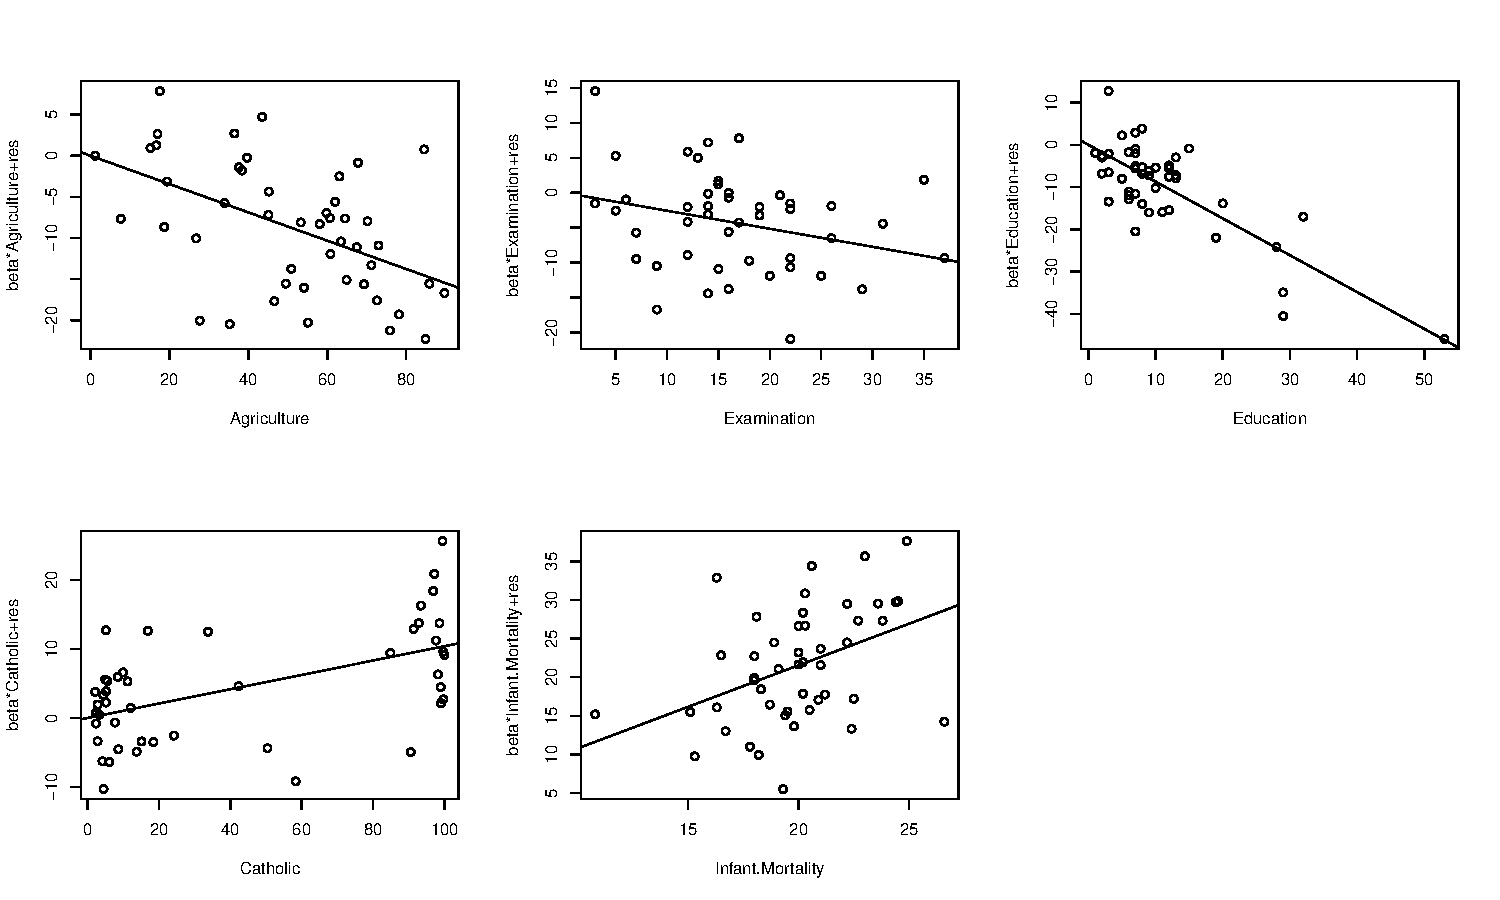
\includegraphics[width=\textwidth]{partial_residual_plots1.pdf}
\end{longproblem}

\problem{ Faraway 4.5.~(pg.~75) For the \texttt{divusa} data, fit a model with
\texttt{divorce} as the response and the other variables except year as predictors. Check for serial correlation.}
\begin{solution}
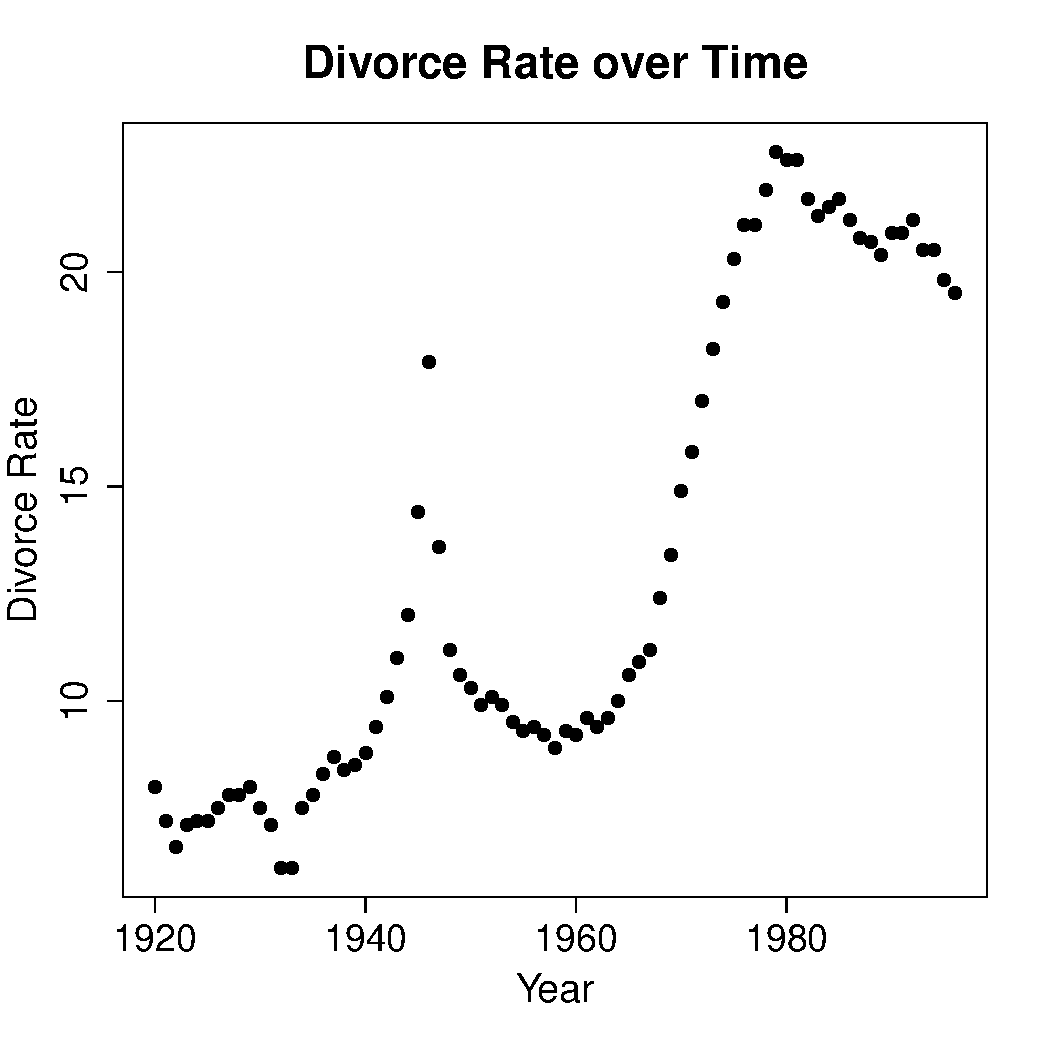
\includegraphics[width=.45\textwidth]{time_plot21.pdf}
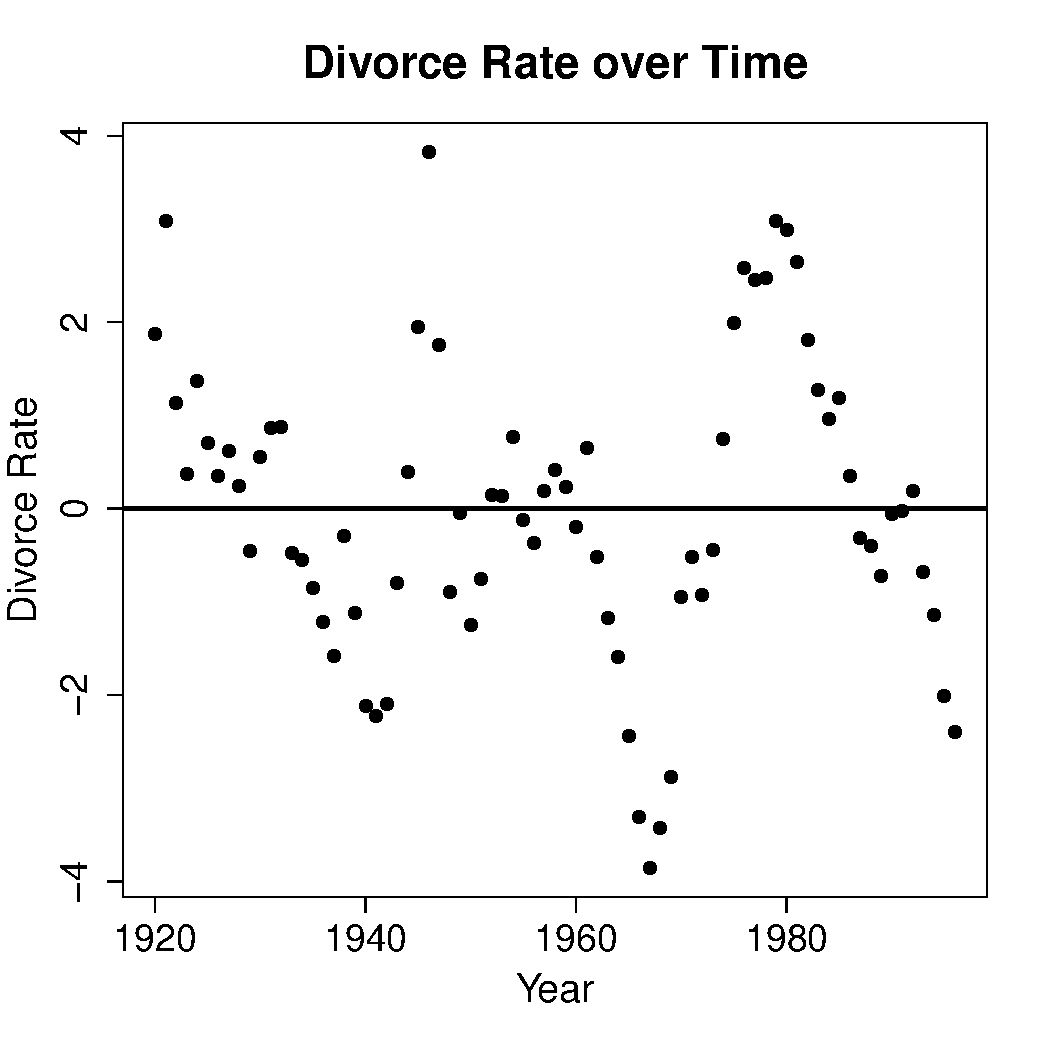
\includegraphics[width=.45\textwidth]{time_plot22.pdf}
  First note the time plots of divorce vs. time and the residuals vs. time indicate that the observations are time dependent.  In particular, divorce first increases, then decreases, then increases dramatically, then seems to level off as time progresses.  This presents itself as an oscillating pattern in the residual plot.

 To formally test for the serial correlation among residuals suggested by the plots, we conduct a Durbin-Watson test  
 $$
  H_0\,:\,\text{The $\epsilon_i$ are not correlated}\quad\text{vs.}\quad H_a\,:\,\text{The $\epsilon_i$ are correlated,}
 $$
 with \texttt{DW = 0.2999, p-value < 2.2e-16}, indicating very strong statistical evidence for correlation.  Since the DW-test requires normality, we verify that the residuals are normal, and indeed a qqplot and the Shapiro-Francia test (\texttt{W = 0.9898, p-value = 0.711}) present no evidence to the contrary.

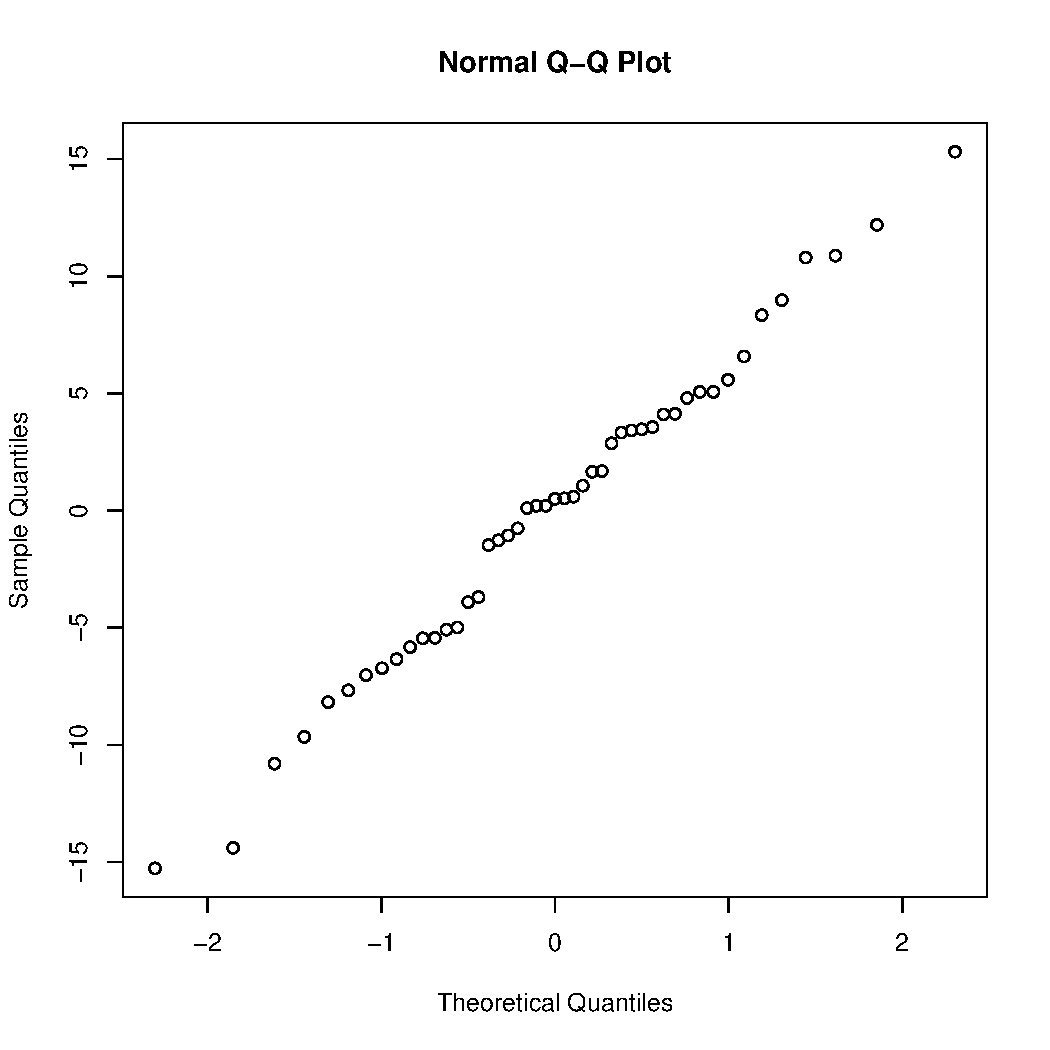
\includegraphics[width=.4\textwidth]{qqplot1.pdf}
\end{solution}

\begin{longproblem}
  Consider the table below of regression diagnostics on the wood data from problem 5 of Homework \#3.  
\begin{center}
\begin{tabular}{c c c c c | c c c c c}
  Obs & $h_i$& $r_i$&$t_i$  & Cook’s $D$ & Obs.& $h_i$ &$r_i$  & ti   & Cook’s D\\
\hline
  1  & 0.085 &  -0.250 &  -0.250 &  0.001 &                29  &  0.069 &  0.270 &  0.260 &  0.001 \\
  2  &  0.055 &  1.340 &  1.350 &  0.021 &                 30  &  0.029 &  0.890 &  0.890 &  0.005 \\
  3  &  0.021 &  0.570 &  0.570 &  0.001 &                 31  &  \a{0.204} &  0.300 &  0.300 &  0.005 \\
  4  &  0.031 &  0.350 &  0.350 &  0.001 &                 32  &  0.057 &  0.380 &  0.370 &  0.002 \\
  5  &  0.032 &  2.190 &  2.280 &  0.032 &                 33  &  0.057 &  0.050 &  0.050 &  0.000 \\
  6  &  0.131 &  0.200 &  0.190 &  0.001 &                 34  &  0.085 &  -2.430 &  -2.560 &  \a{0.109} \\
  7  &  0.027 &  1.750 &  1.790 &  0.017 &                 35  &  \a{0.186} &  -2.170 &  -2.260 &  \a{0.215} \\
  8  &  0.026 &  1.230 &  1.240 &  0.008 &                 36  &  \a{0.184} &  1.010 &  1.010 &  0.046 \\
  9  &  \a{0.191} &  0.520 &  0.520 &  0.013 &             37  &  0.114 &  0.850 &  0.850 &  0.019 \\
  10 &  0.082 &  0.470 &  0.460 &  0.004 &                 38  &  0.022 &  0.190 &  0.190 &  0.000 \\
  11 &  0.098 &  \a{-3.390} &  \a{-3.820} &  \a{0.250} &           39  &  0.022 &  -0.450 &  -0.450 &  0.001 \\
  12 &  0.066 &  0.320 &  0.320 &  0.001 &                 40  &  0.053 &  -1.150 &  -1.150 &  0.015 \\
  13 &  0.070 &  -0.090 &  -0.090 &  0.000 &               41  &  0.053 &  0.780 &  0.780 &  0.007 \\
  14 &  0.059 &  0.080 &  0.080 &  0.000 &                 42  &  0.136 &  -0.770 &  -0.760 &  0.018 \\
  15 &  0.058 &  -0.910 &  -0.910 &  0.010 &               43  &  0.072 &  -0.780 &  -0.770 &  0.009 \\
  16 &  0.085 &  -0.090 &  -0.090 &  0.000 &               44  &  0.072 &  -0.270 &  -0.260 &  0.001 \\
  17 &  0.113 &  1.280 &  1.290 &  0.042 &                 45  &  0.072 &  -0.400 &  -0.400 &  0.002 \\
  18 &  0.077 &  -1.050 &  -1.050 &  0.018 &               46  &  0.063 &  -0.620 &  -0.620 &  0.005 \\
  19 &  0.167 &  0.380 &  0.380 &  0.006 &                 47  &  0.025 &  0.460 &  0.460 &  0.001 \\
  20 &  0.042 &  0.240 &  0.230 &  0.000 &                 48  &  0.021 &  0.180 &  0.180 &  0.000 \\
  21 &  \a{0.314} &  -0.190 &  -0.190 &  0.003 &           49  &  0.050 &  -0.440 &  -0.440 &  0.002 \\
  22 &  0.099 &  0.560 &  0.550 &  0.007 &                 50  &  0.161 &  -0.660 &  -0.660 &  0.017 \\
  23 &  0.093 &  0.470 &  0.460 &  0.004 &                 51  &  0.042 &  -0.440 &  -0.430 &  0.002 \\
  24 &  0.039 &  -0.600 &  -0.600 &  0.003 &               52  &  0.123 &  -0.260 &  -0.260 &  0.002 \\
  25 &  0.098 &  -1.070 &  -1.070 &  0.025 &               53  &  \a{0.460} &  1.810 &  1.860 &  \a{0.558} \\
  26 &  0.033 &  0.140 &  0.130 &  0.000 &                 54  &  0.055 &  0.500 &  0.500 &  0.003 \\
  27 &  0.042 &  1.190 &  1.190 &  0.012 &                 55  &  0.093 &  -1.030 &  -1.030 &  0.022 \\
  28 &  \a{0.185} &  -1.410 &  -1.420 &  \a{0.090} & & & & & \\
\hline
Cutoff & 0.182 &  &  3.532 & 0.073 & & 0.182 &  &  3.532 & 0.073 \\

 \end{tabular} 
\end{center}

  \subproblem{ Are there any unusual values in the predictor variables?  In other words, do any of the values have unusually large influence on the model?  Identify all such cases and explain your reasoning. }

  Observations 53, 21, and 31 have very high leverage values and thus have great influence on the model.  Note also that observations 9, 28, 35, and 36 also have leverages above the rule of thumb given in 5d, hence may have greater than usual influence on the model. 

  \subproblem{ Identify any model outliers in these data, clearly explaining your reasoning. }

  Outliers were tested by finding those with $t_i$ whose magnitude was greater than the 95\% Bonferroni corrected $t_{.05/2\cdot n}(n-p-1)=3.532$.  Observation 55 has statistical evidence for being an outlier.  Note that observations 34, 35, and 5 also have large studentized residuals, but are not statistically significant outliers.
\newpage

  \subproblem{ Which observations are most influential in terms of the predictive ability of the model? Explain your reasoning clearly }

  For determining the predictive influence, we find those
  observations whose Cooks' D statistic is greater than $4/n$.  The
  outlying observation 11 is highly influential by this standard, as
  is the previously mentioned obs.~53.  Others that are also above
  the cutoff are 35, 34, and 28.
\end{longproblem}

\begin{longproblem}
  There have been numerous efforts to collect data which support or refute the theory of global warming.  This problem considers a data set containing the temperature in degrees Celsius averaged for the northern hemisphere over a full year, from 1881 through 2005.  The data can be found in the data file \texttt{warming2005.txt} on the course webpage. [Data from K.M. Lugina et al., 2006. Monthly surface In Trends Online:  A compendium of Data on Global Change.  Carbon Diode Information Analysis Center, Oak Ridge National Laboratory, U.S. Department of Energy.  Oak Ridge, Tennessee, U.S.A.doi:10.3334/CDIAC/cli.003.]
  
  \subproblem{ Make a scatterplot of temperature vs.~time and fit a single linear regression model with temperature as the response variable.  Test for an \emph{increase} in temperature over time.  Explain your conclusions.}

\begin{minipage}{.4\textwidth}
  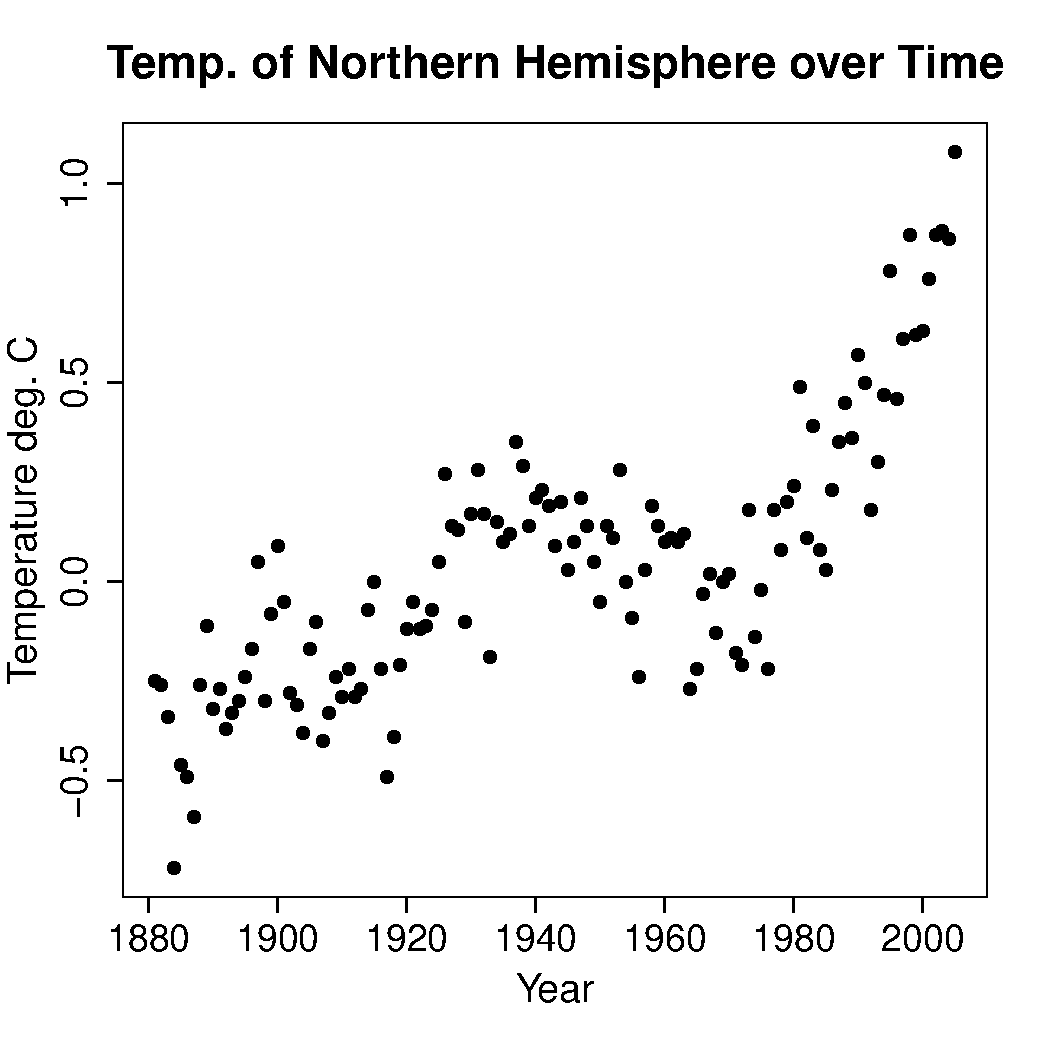
\includegraphics[width=\textwidth]{time_plot4.pdf}
\end{minipage}
\begin{minipage}{.6\textwidth}
  We fit the model $y_i = \beta_0 + \beta_1 x_i + \epsilon_i$, where $y_i$ is the temperature and $x_i$ is the year. We test the hypothesis $$
  H_0:\beta_1 = 0\quad\text{ vs. }H_a:\beta_1 > 0
$$
using normal inference for $\hat \beta_1$ for testing for an increase in tempearture. There is very strong evidence ($t = 13.46$, $p < 1\times10^{-16}$)  for the increase.  Despite apparent non-linear, the best fit line to the data is has a clearly positive slope.  Moreover $n=125$ reduces the standard error for $\beta_1$, effectively inflating $p$ value.
\end{minipage}

  \subproblem{ Inherent with the test in part (a) are a number of assumptions.  One of these is that of normality of the errors.  Make a normal quantile plot of the residuals.  Just looking at the plot, do these data appear to violate the normality assumption?  Test for normality of the residuals using a normal scores correlation (Shapiro-Francia) test.}
\begin{minipage}{.35\textwidth}
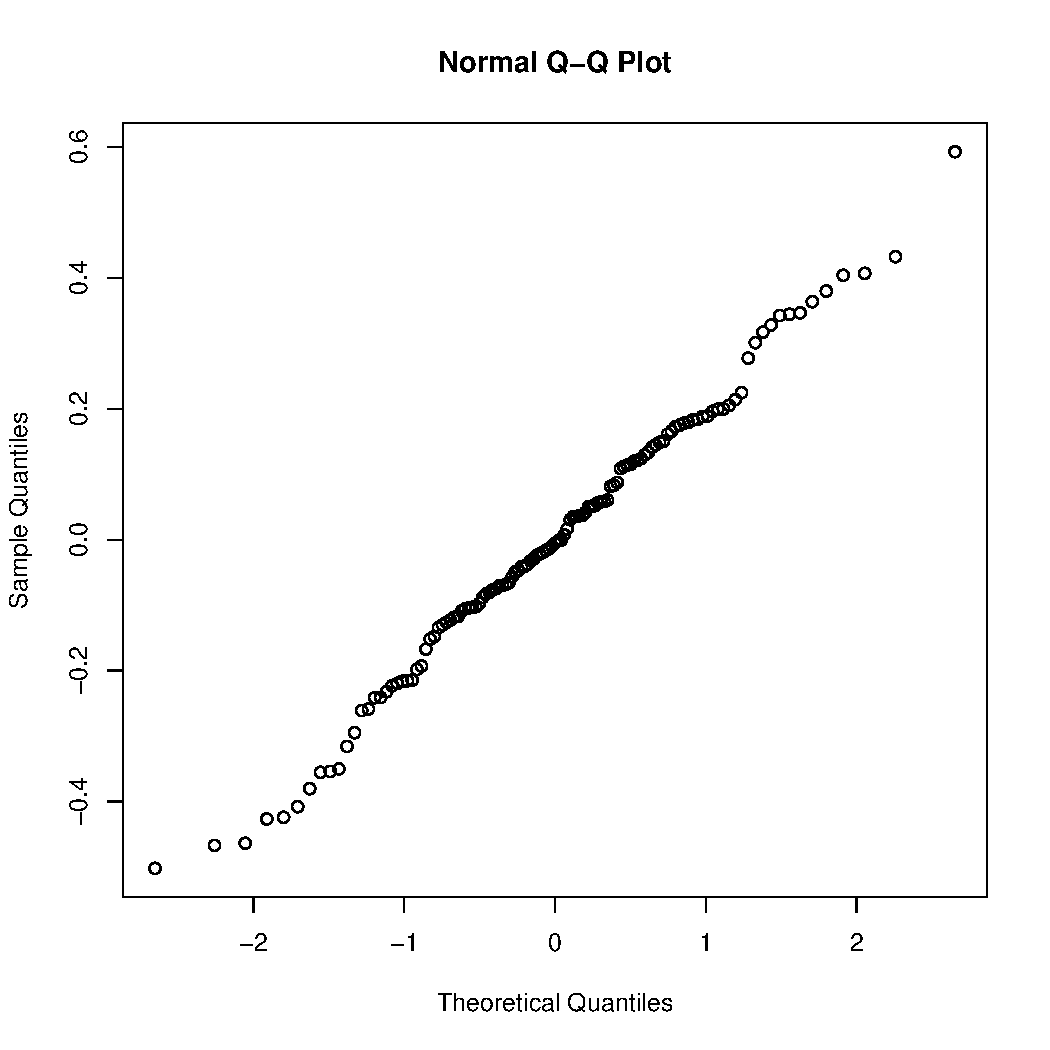
\includegraphics[width=\textwidth]{qqplot4.pdf}
\end{minipage}
\begin{minipage}{.6\textwidth}
  There is no convincing evidence of non-normality in the qqplot, and this is confirmed by the Shapiro-Francia test: \texttt{W = 0.9928, p-value = 0.6809}.
\end{minipage}
\newpage

  \subproblem{Using the unstandardized residuals found in part (b), make a plot of the residuals vs.~time. Just looking at this plot, does there appear to be any serial correlation?  Explain. Test for the presence of serial correlation using a Durbin-Watson test.  [In \texttt{R}, you can request the Durbin-Watson test using the \texttt{dwtest} function in the package \texttt{lmtest} as illustrated in class.}

\begin{minipage}{.35\textwidth}
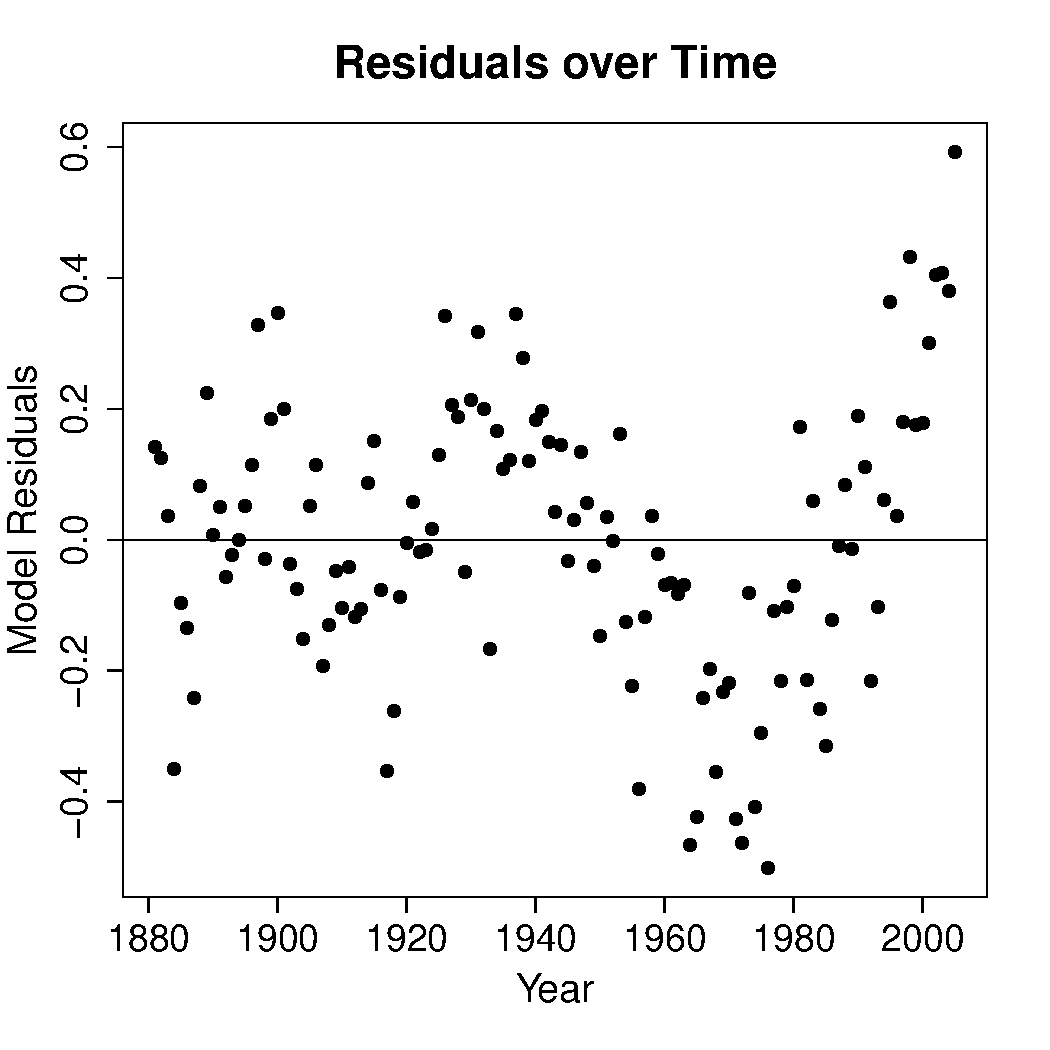
\includegraphics[width=\textwidth]{resid4.pdf}
\end{minipage}
\begin{minipage}{.6\textwidth}
  There is a clear oscillating pattern as the residuals increase in time.  This indicates that there is dependence between sequential observations, i.e. serial correlation.  We formally test this with the Durbin-Watson test
 $$
  H_0\,:\,\text{The $\epsilon_i$ are not correlated}\quad\text{vs.}\quad H_a\,:\,\text{The $\epsilon_i$ are correlated,}
 $$
  with \texttt{DW = 0.706, p-value = 7.598e-14} indicating very strong evidence for correlation.  
\end{minipage}

  \subproblem{Test for serial correlation using a runs test.  What is the p-value for this test? [In \texttt{R}, you can perform a runs test using the \texttt{runs.test} function in the \texttt{tseries} package as shown in the \texttt R-code from the Diagnostics handout on the course webpage.]}

  The non-parametric runs-test tests for the presence of positive or negative serial correlation.  The results are \texttt{Standard Normal = -4.7494, p-value = 2.04e-06}, indicating strong evidence for the presence of serial correlation.

\end{longproblem}

\begin{longproblem}
  Data were collected from 60 major US cities to study the relationship between mortality rates and air pollution.  Letting the response variable be total age-adjusted mortality rate per 100,000 people for a city, the following predictor variables were considered: mean annual precipitation in inches ($x_1$), mean January temperature in degrees F ($x_2$), mean July temperature in degrees F ($x_3$), population per household ($x_4$), median school years completed by those over the age of 25 ($x_5$), percent of housing units that are sound and with all facilities ($x_6$), population per square mile in urbanized areas ($x_7$), percent non-white population in urbanized areas ($x_8$), relative pollution potential of sulphur dioxide ($x_9$), and annual average of percent relative humidity at 1pm ($x_{10}$).  These data can be found in the file \texttt{pollution.txt} on the course webpage.  Using only the variables $y,x_2,x_4,x_5$ and $x_7$ (to keep things manageable), carry out the following.

  \subproblem{ Make pairwise scatterplots and compute the matrix of sample correlations between the 5 variables.  In a paragraph, briefly describe any apparent relationships between the variables and the nature of those relationships, based on the plots and correlations.}

  \begin{minipage}{.5\textwidth}
  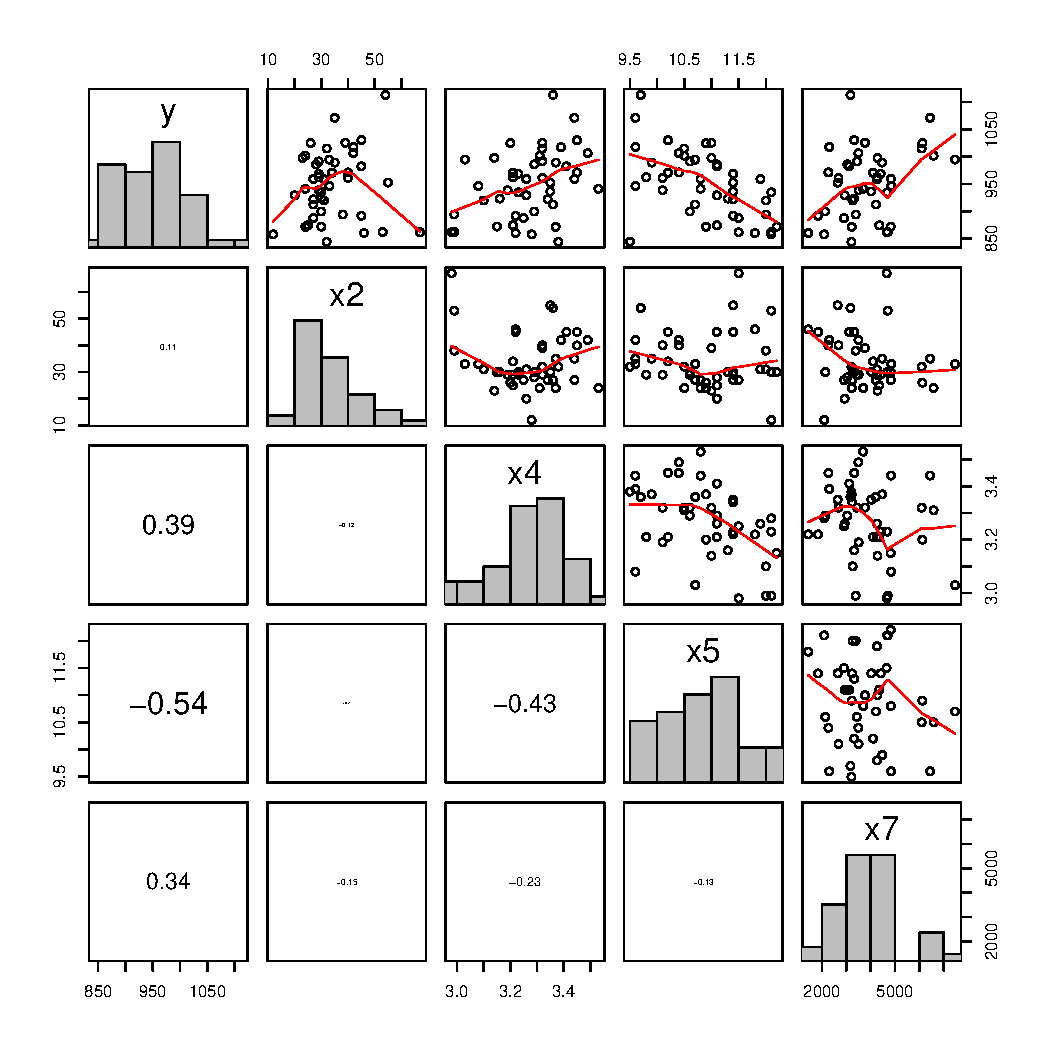
\includegraphics[width=\textwidth]{pollution_pairs.pdf}
  \end{minipage}
  \begin{minipage}{.5\textwidth}
    There appears to be no relationship with $x_2$, a positive relationship with
    $x_4$ and $x_7$, and a negative relationship with $x_5$.  From the scatter
    plots there appears to be no serious issues with correlations.  The
    correlations are given in the graphic to the left scaled to their relative
    size.  These indicate potential collinearity between $x_4$ and $x_5$ ($r =
    -0.43$).
  \end{minipage}

  \subproblem{ Construct a table similar to the one given in the Chapter 8 class notes containing the $R^2$, $R_{adj}^2, C_p, \sqrt{\MSE}, \mathrm{AIC},$ and PRESS statistics for \emph{all} possible first-order models using those above. [Note: there are 4, 6, 4, \& 1 models with 1, 2, 3, \& 4 predictors in them respectively, for a total of 15 models.] Interpret this table.  Do the selection criteria for finding the ``best model'' agree?  Which model seems best (based on the four explanatory variables used)?}
 {\footnotesize 
  \begin{center}
  \begin{tabular}{c | l l l l l l l }
  Model & $R^2$ & $R^2_{adj}$ & $C_p$ & $\sqrt{\MSE}$ & AIC & BIC & PRESS \\\hline
  $x_2+x_4+x_5+x_7$ &  0.478 & \a{0.425} & \a{5} & \a{46.4} & \a{350} & 359 & 1.14e+05 \\        
  $x_4+x_5+x_7$     &  0.44 & 0.399 & \a{5.89} & 47.4 & 351 & \a{358} & \a{1.1e+05} \\      
  $x_2+x_5+x_7$     &  0.381 & 0.336 & 10.4 & 49.9 & 356 & 363 & 1.34e+05 \\    
  $x_2+x_4+x_7$     &  0.405 & 0.361 & 8.59 & 48.9 & 354 & 361 & 1.25e+05 \\    
  $x_2+x_4+x_5$     &  0.336 & 0.288 & 13.8 & 51.6 & 359 & 366 & 1.35e+05 \\    
  $x_5+x_7$         &  0.365 & 0.335 & 9.62 & 49.9 & 355 & 360 & 1.22e+05 \\    
  $x_4+x_5$         &  0.323 & 0.291 & 12.8 & 51.5 & 358 & 363 & 1.29e+05 \\    
  $x_4+x_7$         &  0.345 & 0.313 & 11.2 & 50.7 & 356 & 362 & 1.2e+05 \\     
  $x_2+x_5$         &  0.3 & 0.267 & 14.6 & 52.4 & 359 & 365 & 1.4e+05 \\       
  $x_2+x_7$         &  0.14 & 0.0992 & 26.8 & 58.1 & 368 & 374 & 1.8e+05 \\     
  $x_2+x_4$         &  0.178 & 0.139 & 23.9 & 56.8 & 366 & 372 & 1.61e+05 \\    
  $x_2$             &  0.0126 & -0.0104 & 34.6 & 61.5 & 373 & 376 & 1.9e+05 \\  
  $x_4$             &  0.153 & 0.133 & 23.9 & 57 & 366 & 369 & 1.52e+05 \\      
  $x_5$             &  0.293 & 0.277 & 13.1 & 52 & 358 & 361 & 1.31e+05 \\      
  $x_7$             &  0.113 & 0.0926 & 26.9 & 58.3 & 368 & 371 & 1.58e+05 \\   
  \end{tabular}
  \end{center}
 }

 Based on the previous table, either the full model or the one with only $x_4,x_5$ and $x_7$ seem to be the best candidates.  Note that there is some disagreement, and those that are known to favor larger $p$ ($R^2_{adj}$, $\sqrt{MSE}$) indeed do. Note also that the $C_p$ statistic that is closest to the line $C_p = p$ are those with $3$ and $4$ parameters.  Since $p=4$ guarantees $C_p = p$, either might be appropriate.  If the goal of the researchers is to predict, $x_2+x_4+x_5+x_7$ is best, but if parsimony is valued, then $x_4+x_5+x_7$ is appropriate. For the remaining problems, we will work with the smaller model. 

  \subproblem{ Perform some residual diagnostics, such as examining residual plots and normal quantile plots for the ``best model'' chosen from part (b).  Draw some conclusions about assumptions on the errors. }

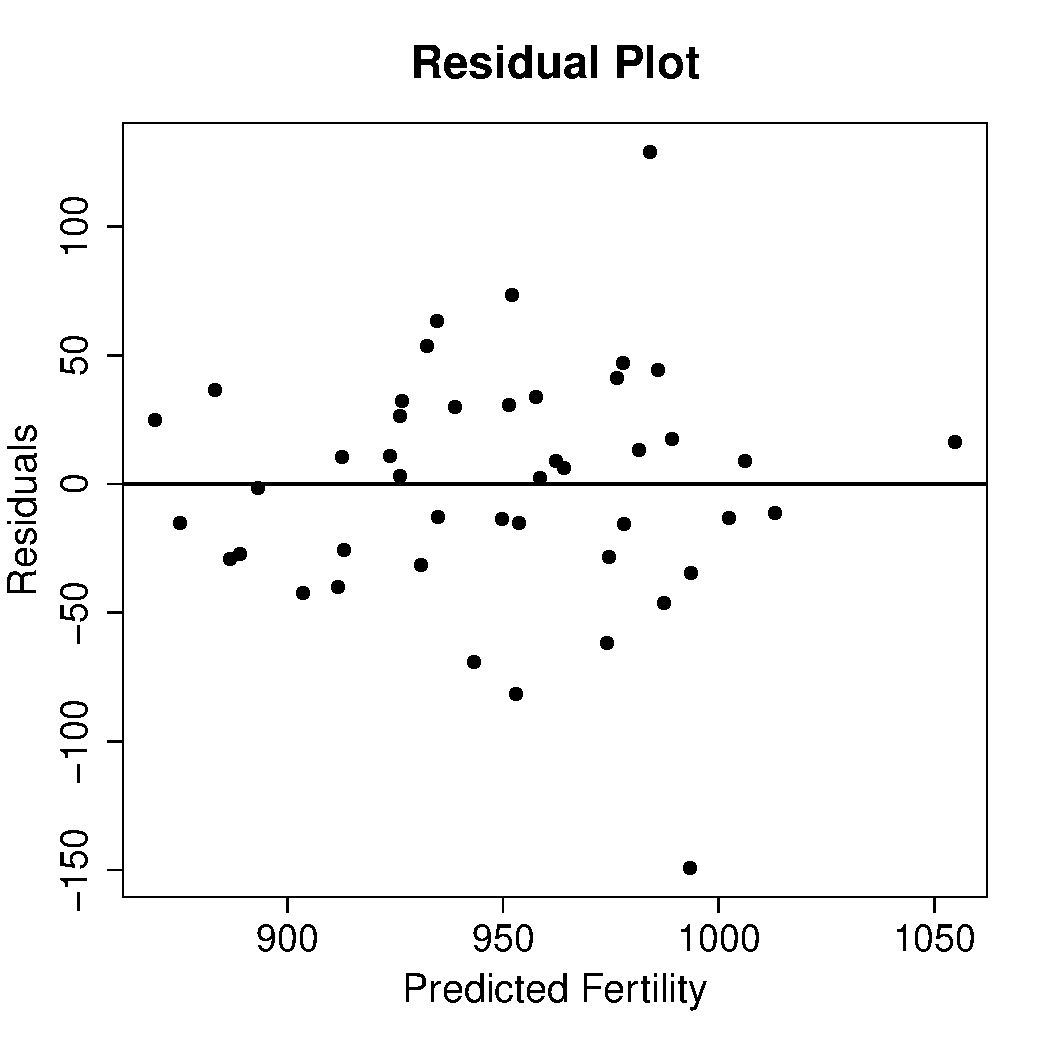
\includegraphics[width=.45\textwidth]{resid5.pdf}
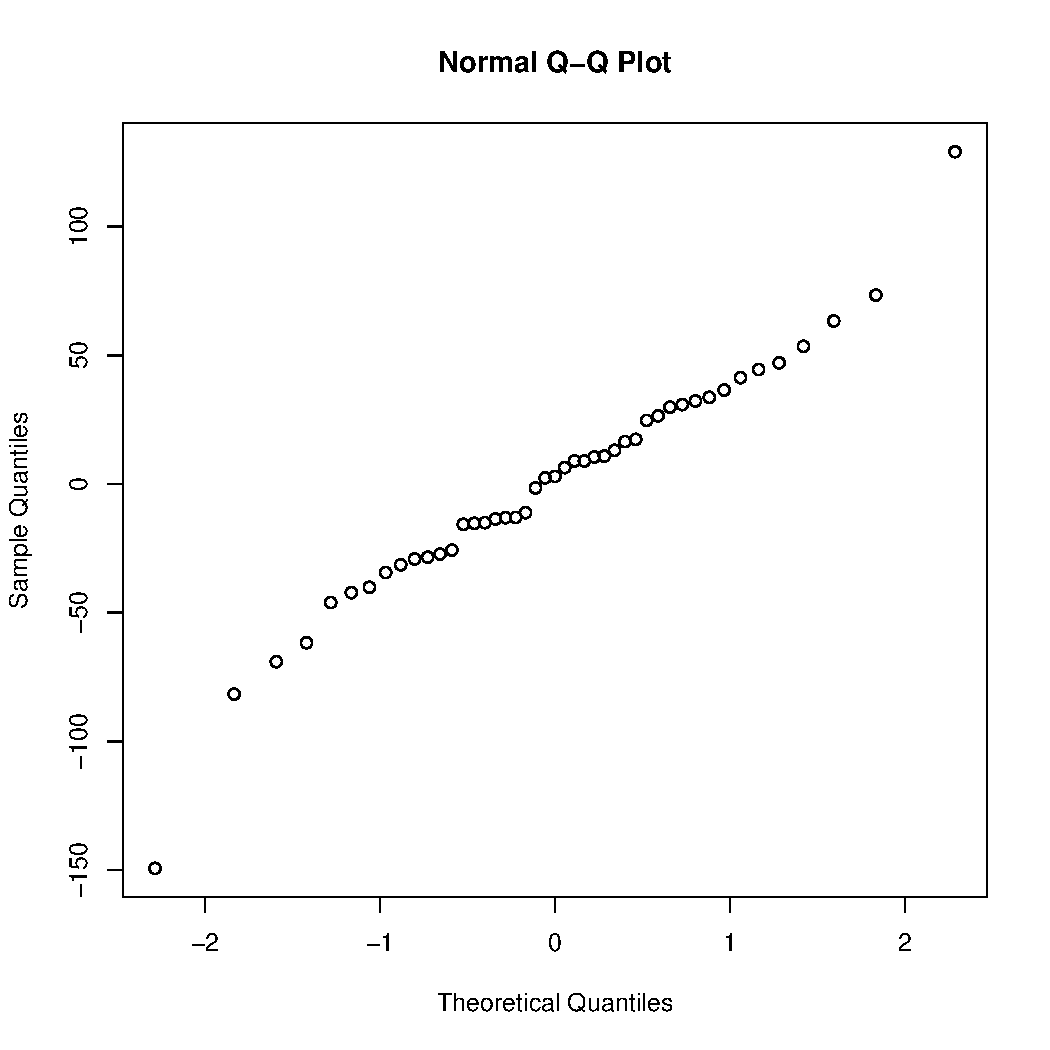
\includegraphics[width=.45\textwidth]{qqplot5.pdf}

From both plots, there appears to be two potentially outlying
values.  One with an abnormally high residual, and one with a low
one. The Shapiro-Francia test for normality indicates evidence for
non-normality (\texttt{W = 0.95, p-value = 0.05}) which may very well be due to the outlying values.  Based on the qqplot, it appears that in the absence of these values the data is reasonably normal.

  \subproblem{ In addition to performing residual diagnostics, it is important to conduct various regression diagnostics to look for outliers or influential data values. Probably the most popular statistics for identifying outlying or influential values are leverage, Cook's D, DFFits, or DFBetas, discussed in class.  Each of these four diagnostic tools can be requested in \texttt R as explained in class or in Section 4.2.3 of the text. Examine the values for the residuals, the leverages, and the three influence statistics resulting from the final model above, and identify any points which would be considered outliers or influential by more than one of the statistics. }
\end{longproblem}

{\small
\begin{center}
\begin{tabular}{c | c c c c c c c}
Obs & $t_i$ & $h_i$ & Cooks' D & DFFits & DFF $x_4$ & DFF $x_5$ & DFF $x_7$ \\ \hline
5 &  0.383 &  \a{0.193} &  0.188 &  -0.049 &  0.080 &  -0.041 &  0.135 \\
20&  -1.040 &  0.128 &  -0.399 &  \a{0.323} & \a{-0.362} & -0.154 &  -0.095 \\
\a{28}&  \a{-3.854} &  0.108 &  \a{-1.340} &  \a{-0.571} & 0.129 &  \a{1.069} & \a{0.466} \\
\a{37}&  3.145 &  0.089 &  \a{0.982} &  \a{0.437} & -0.126 &  \a{-0.763} & \a{-0.383} \\
38&  0.313 &  \a{0.238} &  0.175 &  0.053 &  -0.070 &  -0.028 &  0.120 \\
43&  -0.671 &  \a{0.215} &  -0.352 &  \a{-0.309} & 0.267 &  0.285 &  0.025 \\ \hline
Cutoff & 3.514 & 0.178 & 0.089 & 0.596 & 0.298& 0.298  & 0.298 \\  
\end{tabular}
\end{center}
}

In the previous table are all the observations with a high studentized residual or any high influence statistic or leverage.  Note that it is observation 28 with the abnormally low residual and observation 37 with the abnormally high one.  The cutoff for $t_i$ is the 95\% Bonferroni corrected value $t_{.05/2\cdot n}(n-p-1)=3.514$, and there is statistical evidence  for obs. 28 to be outlying.  Observations 20 and 43 are also influential as they have two influence statistics above the recommended cutoffs.
\newpage

\begin{longproblem}
Faraway 8.3. Use the \texttt{divusa} dataset with \texttt{divorce} as the response and the other variables as predictors. Implement the following variable selection methods to determine the ``best'' model:

  \subproblem{ Backward Elimination }
  \subproblem{ AIC }
  \subproblem{ Adjusted $R^2$ }
  \subproblem{ Mallows $C_p$ }
\end{longproblem}
\begin{solution}
  For part (a), we use the \texttt{regsubsets} function in the \texttt{leaps} library with the option \texttt{method="backwards"} to obtain the best 2,3,4,5,6 and 7 parameter models.  Denote Y = year, U = unemployed, F = femlab, $\heartsuit$ = marriage, B = birth, M = military, and backwards elimination results in

  \begin{tabular}{c l}
 1& Y,U,F,$\heartsuit$,B,M\\
 2& Y,F,$\heartsuit$,B,M\\
 3& Y,F,$\heartsuit$,B\\
 4& F,$\heartsuit$,B\\
 5& F,B\\
 6& F\\
  \end{tabular}

  Now, to determine the best model of these, we calculate the model selection critera in (b)-(d).  The results are summarized in the following table.

  \begin{tabular}{l| c c c c }
  Model & AIC & $R^2_{adj}$ & $C_p$ & $p$ \\ \hline
  Y,U,F,$\heartsuit$,B,M  &  70.41 & 0.9288 & 7 & 7 \\ 
  \a{Y,F,$\heartsuit$,B,M}    &  \a{69.33} & \a{0.929} & \a{5.841} & 6 \\ 
  Y,F,$\heartsuit$,B      &  76.69 & 0.9209 & 13 & 5 \\ 
  F,$\heartsuit$,B        &  85.2 & 0.9106 & 22.69 & 4 \\ 
  F,B                     &  111.8 & 0.872 & 62 & 3 \\ 
  F                       &  134.3 & 0.8265 & 109.7 & 2 \\ 
  \end{tabular}

  In each case, the 6 parameter model is selected to be ``best''. To see this for $C_p$, note that the $C_p=p$ line first crosses between the 6 and 7 parameter model and is closest to the 6 parameter one.   
  
  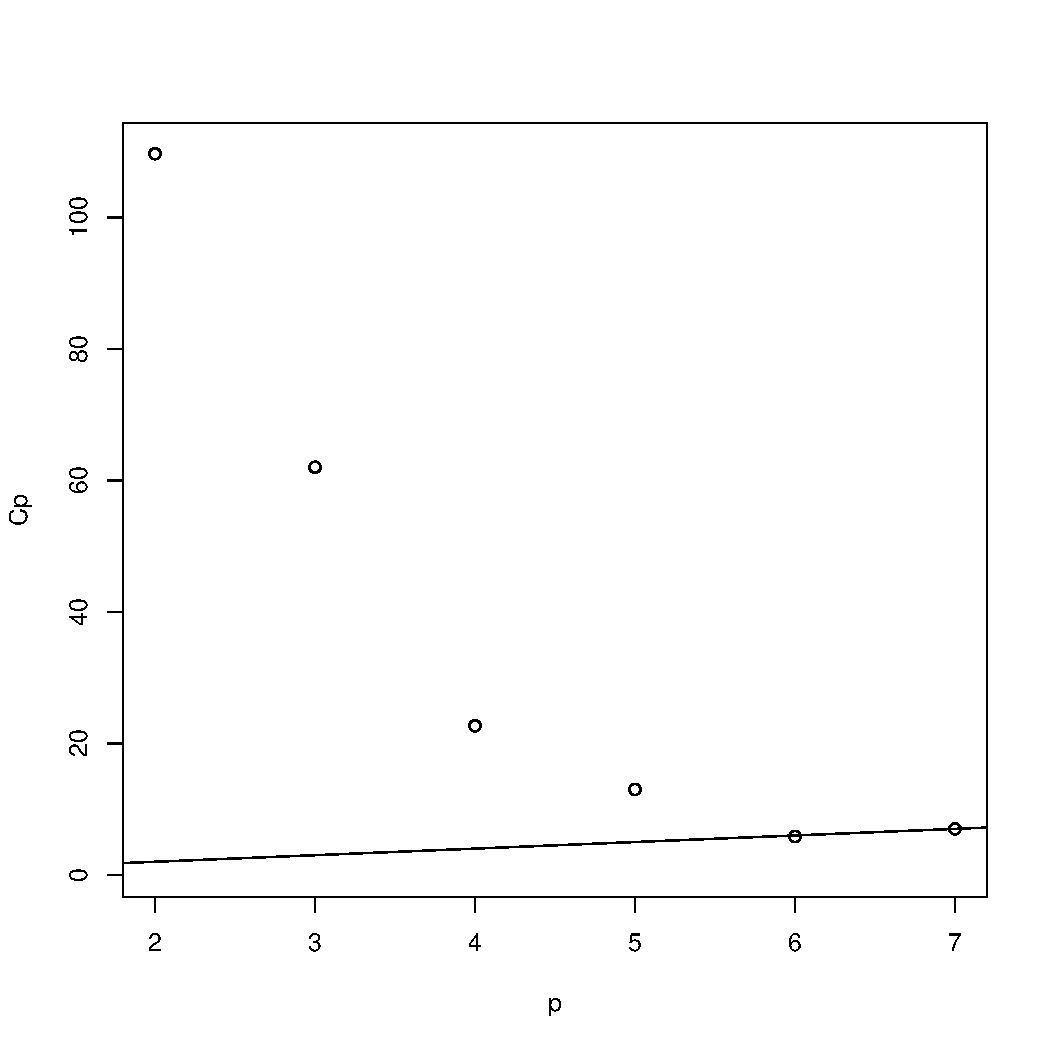
\includegraphics[width=.4\textwidth]{cp_line.pdf}
\end{solution}
\end{document} 

